% ------------------------------------------------------------------------
% ------------------------------------------------------------------------
% ------------------------------------------------------------------------
%                                Capítulo 4
% ------------------------------------------------------------------------
% ------------------------------------------------------------------------
% ------------------------------------------------------------------------

\chapter{Resultados}

Para evaluar el método propuesto se presentan los siguientes experimentos realizados. 

\section{Conjuntos de datos}

Durante el desarrollo de este trabajo, no se encontraron conjuntos de datos públicos enfocados en la clasificación de medidas cuadráticas. Debido a esto, se decidió simular la propagación de las medidas usando conjuntos de datos tradicionales. Para esto se usaron imágenes de los conjuntos de datos MNIST \myfootcite{deng2012mnist} y Fashion-MNIST \myfootcite{xiao2017fashion}. La Figura \ref{fig:conjunto_datos} muestra un ejemplo de diferentes La Tabla \ref{tab:conjunto_datos} muestra la división de datos en entrenamiento, validación y prueba. Cada imagen fue escalada en el rango de $[-\pi, \pi]$ y usada como información de fase de la forma $\mathbf{x}=e^{j\mathrm{ang}(\mathbf{x})}$, donde $j$ representa la unidad imaginaria en el plano complejo.

\begin{figure}[!h]
    \centering
    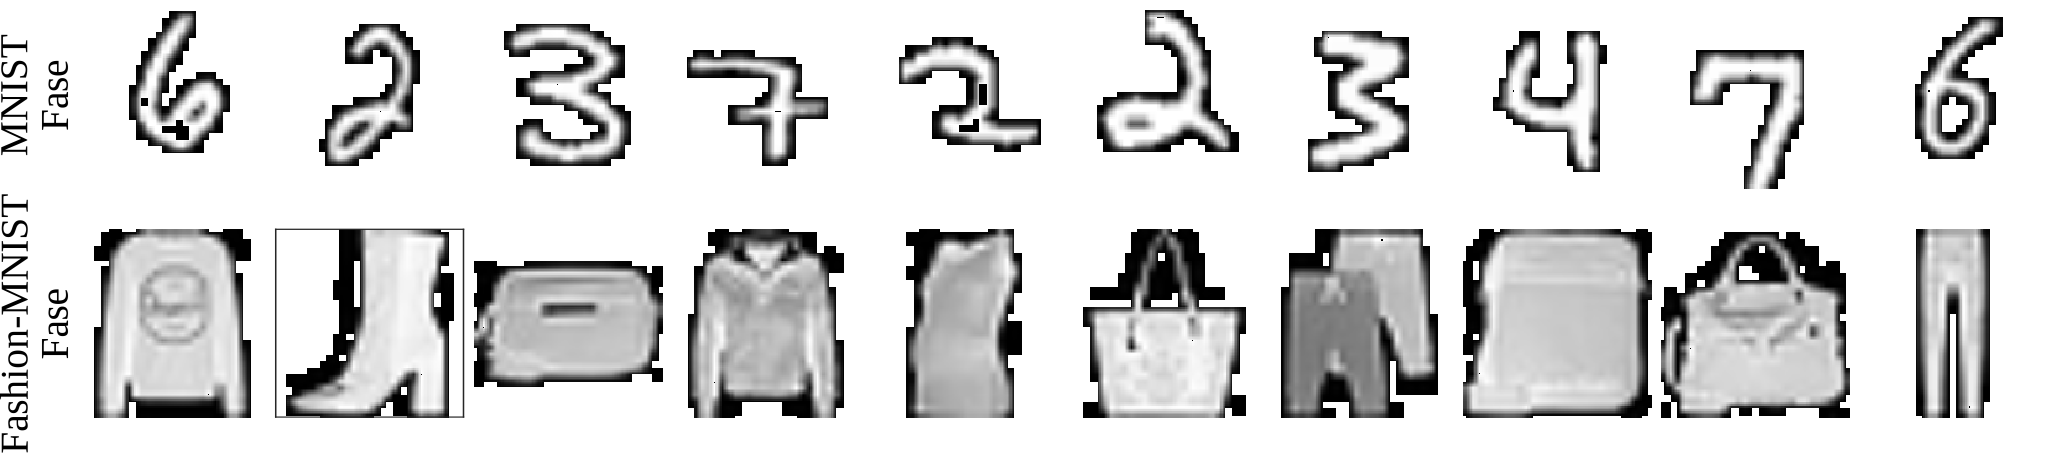
\includegraphics[width=\linewidth]{images/datasets.pdf}
    \caption{Ejemplo de las imágenes presentes en los conjuntos de datos MNIST y Fashion-MNIST.}
    \label{fig:conjunto_datos}
\end{figure}


% Please add the following required packages to your document preamble:
% \usepackage{graphicx}
\begin{table}[!h]
\centering\scalebox{0.9}{
\resizebox{\textwidth}{!}{%
\begin{tabular}{|c|c|c|c|c|}
\hline
\textbf{Conjunto de datos} & \textbf{Entrenamiento} & \textbf{Validación} & \textbf{Prueba} & \textbf{Total} \\ \hline
MNIST                      & 54000                  & 6000                & 10000           & 70000          \\ \hline
Fashion-MNIST              & 54000                  & 6000                & 10000           & 70000          \\ \hline
\end{tabular}%
}}\caption{Resumen de la división de los conjuntos de datos usados para evaluar el método propuesto.}
\label{tab:conjunto_datos}
\end{table}

\section{Métricas}

\begin{itemize}
    \item Accuracy
    \item Métrica-F1
\end{itemize}





\section{Experimentos}

\subsection{Comparación con el Estado del arte}

\begin{itemize}
    \item Es el esquema de clasificación directamente sobre las medidas sin usar codificación
\end{itemize}

\subsection{Configuración hiperparámetros}
\begin{itemize}
    \item 
    \item 
\end{itemize}

\subsection{Validación cruzada}

\begin{itemize}
    \item Quisimos verificar si los resultados variaban mucho según la porción del dataset bla bla bla
\end{itemize}


% Please add the following required packages to your document preamble:
% \usepackage{multirow}
% \usepackage{graphicx}
\begin{table}[!h]
\centering
\resizebox{\textwidth}{!}{%
\begin{tabular}{|c|ccc|ccc|ccc|}
\hline
\multirow{2}{*}{Metric} &
  \multicolumn{3}{c|}{Near-field} &
  \multicolumn{3}{c|}{Middle-field} &
  \multicolumn{3}{c|}{Far-field} \\ \cline{2-10} 
 &
  \multicolumn{1}{c|}{None} &
  \multicolumn{1}{c|}{Back} &
  FSI &
  \multicolumn{1}{c|}{None} &
  \multicolumn{1}{c|}{Back} &
  FSI &
  \multicolumn{1}{c|}{None} &
  \multicolumn{1}{c|}{Back} &
  FSI \\ \hline
Accuracy &
  \multicolumn{1}{c|}{$0.5 pm 0.27$} &
  \multicolumn{1}{c|}{$0.48 pm 0.29$} &
  $0.62 pm 0.33$ &
  \multicolumn{1}{c|}{$0.44 pm 0.3$} &
  \multicolumn{1}{c|}{$0.67 pm 0.33$} &
  $0.55 pm 0.25$ &
  \multicolumn{1}{c|}{$0.51 pm 0.33$} &
  \multicolumn{1}{c|}{$0.67 pm 0.24$} &
  $0.46 pm 0.32$ \\ \hline
F1-Score &
  \multicolumn{1}{c|}{$0.5 pm 0.27$0} &
  \multicolumn{1}{c|}{$0.5 pm 0.27$1} &
  $0.5 pm 0.27$2 &
  \multicolumn{1}{c|}{$0.5 pm 0.27$3} &
  \multicolumn{1}{c|}{$0.5 pm 0.27$4} &
  $0.5 pm 0.27$5 &
  \multicolumn{1}{c|}{$0.5 pm 0.27$6} &
  \multicolumn{1}{c|}{$0.5 pm 0.27$7} &
  $0.5 pm 0.27$8 \\ \hline
\end{tabular}%
}
\end{table}


\subsection{Resultados principales}

\begin{figure*}[!h]
    \centering
    \includegraphics[width=\linewidth]{images/test_result_f1_score.pdf}
    \caption{Resultados métrica F1-score.}
    \label{fig:results1}
\end{figure*}

\begin{figure*}[!h]
    \centering
    \includegraphics[width=\linewidth]{images/test_result_f1_score.pdf}
    \caption{Resultados métrica F1-score.}
    \label{fig:results2}
\end{figure*}

